% Created by tikzDevice version 0.12.3.1 on 2021-03-01 17:48:53
% !TEX encoding = UTF-8 Unicode
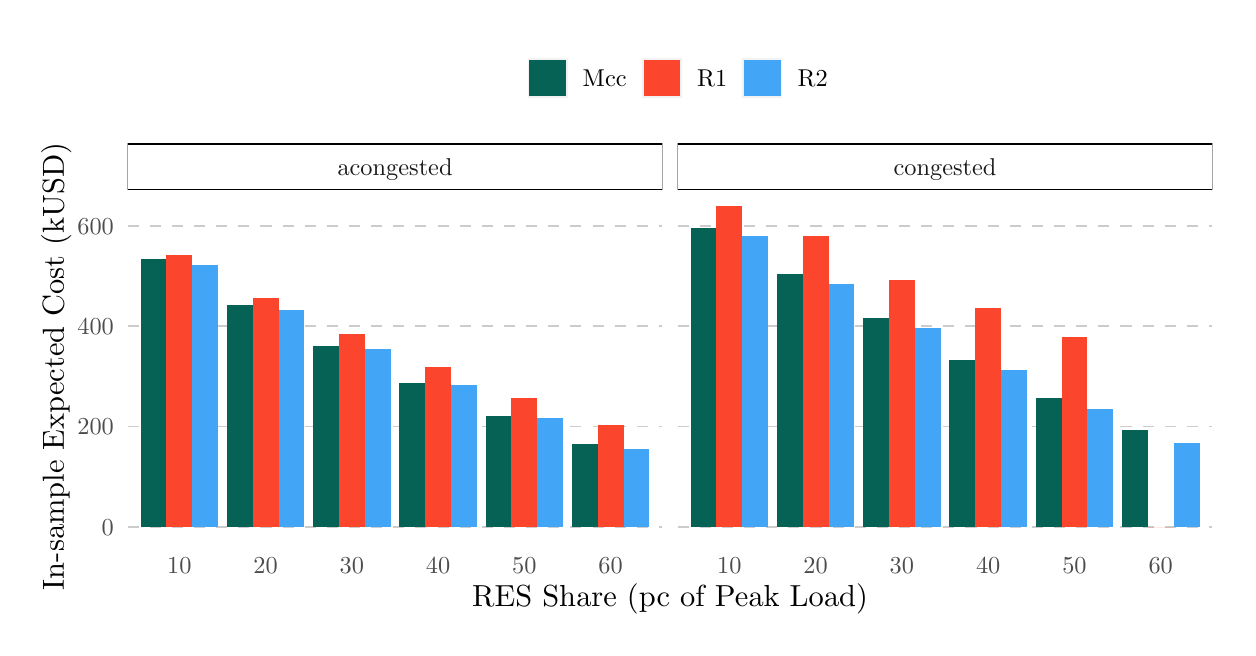
\begin{tikzpicture}[x=1pt,y=1pt]
\definecolor{fillColor}{RGB}{255,255,255}
\path[use as bounding box,fill=fillColor,fill opacity=0.00] (0,0) rectangle (433.62,216.81);
\begin{scope}
\path[clip] (  0.00,  0.00) rectangle (433.62,216.81);

\path[] (  0.00,  0.00) rectangle (433.62,216.81);
\end{scope}
\begin{scope}
\path[clip] ( 36.11, 30.69) rectangle (229.37,158.28);

\path[] ( 36.11, 30.69) rectangle (229.37,158.28);
\definecolor{drawColor}{RGB}{255,255,255}

\path[draw=drawColor,line width= 0.3pt,line join=round] ( 36.11, 54.59) --
	(229.37, 54.59);

\path[draw=drawColor,line width= 0.3pt,line join=round] ( 36.11, 90.81) --
	(229.37, 90.81);

\path[draw=drawColor,line width= 0.3pt,line join=round] ( 36.11,127.03) --
	(229.37,127.03);
\definecolor{drawColor}{gray}{0.80}

\path[draw=drawColor,line width= 0.6pt,dash pattern=on 4pt off 4pt ,line join=round] ( 36.11, 36.49) --
	(229.37, 36.49);

\path[draw=drawColor,line width= 0.6pt,dash pattern=on 4pt off 4pt ,line join=round] ( 36.11, 72.70) --
	(229.37, 72.70);

\path[draw=drawColor,line width= 0.6pt,dash pattern=on 4pt off 4pt ,line join=round] ( 36.11,108.92) --
	(229.37,108.92);

\path[draw=drawColor,line width= 0.6pt,dash pattern=on 4pt off 4pt ,line join=round] ( 36.11,145.14) --
	(229.37,145.14);
\definecolor{fillColor}{RGB}{7,98,86}

\path[fill=fillColor] ( 40.79, 36.49) rectangle ( 50.14,133.30);
\definecolor{fillColor}{RGB}{252,69,45}

\path[fill=fillColor] ( 50.14, 36.49) rectangle ( 59.49,134.49);
\definecolor{fillColor}{RGB}{66,165,245}

\path[fill=fillColor] ( 59.49, 36.49) rectangle ( 68.84,131.23);
\definecolor{fillColor}{RGB}{7,98,86}

\path[fill=fillColor] ( 71.96, 36.49) rectangle ( 81.31,116.71);
\definecolor{fillColor}{RGB}{252,69,45}

\path[fill=fillColor] ( 81.31, 36.49) rectangle ( 90.66,119.25);
\definecolor{fillColor}{RGB}{66,165,245}

\path[fill=fillColor] ( 90.66, 36.49) rectangle (100.01,114.66);
\definecolor{fillColor}{RGB}{7,98,86}

\path[fill=fillColor] (103.13, 36.49) rectangle (112.48,101.95);
\definecolor{fillColor}{RGB}{252,69,45}

\path[fill=fillColor] (112.48, 36.49) rectangle (121.83,106.27);
\definecolor{fillColor}{RGB}{66,165,245}

\path[fill=fillColor] (121.83, 36.49) rectangle (131.18,100.70);
\definecolor{fillColor}{RGB}{7,98,86}

\path[fill=fillColor] (134.30, 36.49) rectangle (143.65, 88.56);
\definecolor{fillColor}{RGB}{252,69,45}

\path[fill=fillColor] (143.65, 36.49) rectangle (153.00, 94.13);
\definecolor{fillColor}{RGB}{66,165,245}

\path[fill=fillColor] (153.00, 36.49) rectangle (162.35, 87.67);
\definecolor{fillColor}{RGB}{7,98,86}

\path[fill=fillColor] (165.47, 36.49) rectangle (174.82, 76.66);
\definecolor{fillColor}{RGB}{252,69,45}

\path[fill=fillColor] (174.82, 36.49) rectangle (184.17, 83.08);
\definecolor{fillColor}{RGB}{66,165,245}

\path[fill=fillColor] (184.17, 36.49) rectangle (193.52, 75.61);
\definecolor{fillColor}{RGB}{7,98,86}

\path[fill=fillColor] (196.64, 36.49) rectangle (205.99, 66.45);
\definecolor{fillColor}{RGB}{252,69,45}

\path[fill=fillColor] (205.99, 36.49) rectangle (215.34, 73.12);
\definecolor{fillColor}{RGB}{66,165,245}

\path[fill=fillColor] (215.34, 36.49) rectangle (224.69, 64.67);
\end{scope}
\begin{scope}
\path[clip] (234.87, 30.69) rectangle (428.12,158.28);

\path[] (234.87, 30.69) rectangle (428.12,158.28);
\definecolor{drawColor}{RGB}{255,255,255}

\path[draw=drawColor,line width= 0.3pt,line join=round] (234.87, 54.59) --
	(428.12, 54.59);

\path[draw=drawColor,line width= 0.3pt,line join=round] (234.87, 90.81) --
	(428.12, 90.81);

\path[draw=drawColor,line width= 0.3pt,line join=round] (234.87,127.03) --
	(428.12,127.03);
\definecolor{drawColor}{gray}{0.80}

\path[draw=drawColor,line width= 0.6pt,dash pattern=on 4pt off 4pt ,line join=round] (234.87, 36.49) --
	(428.12, 36.49);

\path[draw=drawColor,line width= 0.6pt,dash pattern=on 4pt off 4pt ,line join=round] (234.87, 72.70) --
	(428.12, 72.70);

\path[draw=drawColor,line width= 0.6pt,dash pattern=on 4pt off 4pt ,line join=round] (234.87,108.92) --
	(428.12,108.92);

\path[draw=drawColor,line width= 0.6pt,dash pattern=on 4pt off 4pt ,line join=round] (234.87,145.14) --
	(428.12,145.14);
\definecolor{fillColor}{RGB}{7,98,86}

\path[fill=fillColor] (239.54, 36.49) rectangle (248.89,144.25);
\definecolor{fillColor}{RGB}{252,69,45}

\path[fill=fillColor] (248.89, 36.49) rectangle (258.24,152.48);
\definecolor{fillColor}{RGB}{66,165,245}

\path[fill=fillColor] (258.24, 36.49) rectangle (267.59,141.61);
\definecolor{fillColor}{RGB}{7,98,86}

\path[fill=fillColor] (270.71, 36.49) rectangle (280.06,127.74);
\definecolor{fillColor}{RGB}{252,69,45}

\path[fill=fillColor] (280.06, 36.49) rectangle (289.41,141.63);
\definecolor{fillColor}{RGB}{66,165,245}

\path[fill=fillColor] (289.41, 36.49) rectangle (298.76,124.16);
\definecolor{fillColor}{RGB}{7,98,86}

\path[fill=fillColor] (301.88, 36.49) rectangle (311.23,111.91);
\definecolor{fillColor}{RGB}{252,69,45}

\path[fill=fillColor] (311.23, 36.49) rectangle (320.58,125.67);
\definecolor{fillColor}{RGB}{66,165,245}

\path[fill=fillColor] (320.58, 36.49) rectangle (329.93,108.25);
\definecolor{fillColor}{RGB}{7,98,86}

\path[fill=fillColor] (333.05, 36.49) rectangle (342.40, 96.84);
\definecolor{fillColor}{RGB}{252,69,45}

\path[fill=fillColor] (342.40, 36.49) rectangle (351.75,115.38);
\definecolor{fillColor}{RGB}{66,165,245}

\path[fill=fillColor] (351.75, 36.49) rectangle (361.10, 93.25);
\definecolor{fillColor}{RGB}{7,98,86}

\path[fill=fillColor] (364.22, 36.49) rectangle (373.57, 82.96);
\definecolor{fillColor}{RGB}{252,69,45}

\path[fill=fillColor] (373.57, 36.49) rectangle (382.92,104.94);
\definecolor{fillColor}{RGB}{66,165,245}

\path[fill=fillColor] (382.92, 36.49) rectangle (392.27, 79.01);
\definecolor{fillColor}{RGB}{7,98,86}

\path[fill=fillColor] (395.39, 36.49) rectangle (404.74, 71.32);
\definecolor{fillColor}{RGB}{252,69,45}

\path[fill=fillColor] (404.74, 36.49) rectangle (414.09, 36.49);
\definecolor{fillColor}{RGB}{66,165,245}

\path[fill=fillColor] (414.09, 36.49) rectangle (423.44, 66.56);
\end{scope}
\begin{scope}
\path[clip] ( 36.11,158.28) rectangle (229.37,174.86);
\definecolor{drawColor}{RGB}{0,0,0}

\path[draw=drawColor,line width= 0.6pt,line join=round,line cap=round] ( 36.11,158.28) rectangle (229.37,174.86);
\definecolor{drawColor}{gray}{0.10}

\node[text=drawColor,anchor=base,inner sep=0pt, outer sep=0pt, scale=  0.88] at (132.74,163.54) {acongested};
\end{scope}
\begin{scope}
\path[clip] (234.87,158.28) rectangle (428.12,174.86);
\definecolor{drawColor}{RGB}{0,0,0}

\path[draw=drawColor,line width= 0.6pt,line join=round,line cap=round] (234.87,158.28) rectangle (428.12,174.86);
\definecolor{drawColor}{gray}{0.10}

\node[text=drawColor,anchor=base,inner sep=0pt, outer sep=0pt, scale=  0.88] at (331.49,163.54) {congested};
\end{scope}
\begin{scope}
\path[clip] (  0.00,  0.00) rectangle (433.62,216.81);
\definecolor{drawColor}{gray}{0.30}

\node[text=drawColor,anchor=base,inner sep=0pt, outer sep=0pt, scale=  0.88] at ( 54.81, 19.68) {10};

\node[text=drawColor,anchor=base,inner sep=0pt, outer sep=0pt, scale=  0.88] at ( 85.98, 19.68) {20};

\node[text=drawColor,anchor=base,inner sep=0pt, outer sep=0pt, scale=  0.88] at (117.15, 19.68) {30};

\node[text=drawColor,anchor=base,inner sep=0pt, outer sep=0pt, scale=  0.88] at (148.32, 19.68) {40};

\node[text=drawColor,anchor=base,inner sep=0pt, outer sep=0pt, scale=  0.88] at (179.49, 19.68) {50};

\node[text=drawColor,anchor=base,inner sep=0pt, outer sep=0pt, scale=  0.88] at (210.66, 19.68) {60};
\end{scope}
\begin{scope}
\path[clip] (  0.00,  0.00) rectangle (433.62,216.81);
\definecolor{drawColor}{gray}{0.30}

\node[text=drawColor,anchor=base,inner sep=0pt, outer sep=0pt, scale=  0.88] at (253.57, 19.68) {10};

\node[text=drawColor,anchor=base,inner sep=0pt, outer sep=0pt, scale=  0.88] at (284.74, 19.68) {20};

\node[text=drawColor,anchor=base,inner sep=0pt, outer sep=0pt, scale=  0.88] at (315.91, 19.68) {30};

\node[text=drawColor,anchor=base,inner sep=0pt, outer sep=0pt, scale=  0.88] at (347.08, 19.68) {40};

\node[text=drawColor,anchor=base,inner sep=0pt, outer sep=0pt, scale=  0.88] at (378.25, 19.68) {50};

\node[text=drawColor,anchor=base,inner sep=0pt, outer sep=0pt, scale=  0.88] at (409.42, 19.68) {60};
\end{scope}
\begin{scope}
\path[clip] (  0.00,  0.00) rectangle (433.62,216.81);
\definecolor{drawColor}{gray}{0.30}

\node[text=drawColor,anchor=base east,inner sep=0pt, outer sep=0pt, scale=  0.88] at ( 31.16, 33.46) {0};

\node[text=drawColor,anchor=base east,inner sep=0pt, outer sep=0pt, scale=  0.88] at ( 31.16, 69.67) {200};

\node[text=drawColor,anchor=base east,inner sep=0pt, outer sep=0pt, scale=  0.88] at ( 31.16,105.89) {400};

\node[text=drawColor,anchor=base east,inner sep=0pt, outer sep=0pt, scale=  0.88] at ( 31.16,142.11) {600};
\end{scope}
\begin{scope}
\path[clip] (  0.00,  0.00) rectangle (433.62,216.81);
\definecolor{drawColor}{RGB}{0,0,0}

\node[text=drawColor,anchor=base,inner sep=0pt, outer sep=0pt, scale=  1.10] at (232.12,  7.64) {RES Share (pc of Peak Load)};
\end{scope}
\begin{scope}
\path[clip] (  0.00,  0.00) rectangle (433.62,216.81);
\definecolor{drawColor}{RGB}{0,0,0}

\node[text=drawColor,rotate= 90.00,anchor=base,inner sep=0pt, outer sep=0pt, scale=  1.10] at ( 13.08, 94.49) {In-sample Expected Cost (kUSD)};
\end{scope}
\begin{scope}
\path[clip] (  0.00,  0.00) rectangle (433.62,216.81);
\definecolor{fillColor}{RGB}{255,255,255}

\path[fill=fillColor] (169.62,185.86) rectangle (294.61,211.31);
\end{scope}
\begin{scope}
\path[clip] (  0.00,  0.00) rectangle (433.62,216.81);
\definecolor{fillColor}{gray}{0.95}

\path[fill=fillColor] (180.62,191.36) rectangle (195.07,205.81);
\end{scope}
\begin{scope}
\path[clip] (  0.00,  0.00) rectangle (433.62,216.81);
\definecolor{fillColor}{RGB}{7,98,86}

\path[fill=fillColor] (181.33,192.07) rectangle (194.36,205.10);
\end{scope}
\begin{scope}
\path[clip] (  0.00,  0.00) rectangle (433.62,216.81);
\definecolor{fillColor}{gray}{0.95}

\path[fill=fillColor] (221.96,191.36) rectangle (236.41,205.81);
\end{scope}
\begin{scope}
\path[clip] (  0.00,  0.00) rectangle (433.62,216.81);
\definecolor{fillColor}{RGB}{252,69,45}

\path[fill=fillColor] (222.67,192.07) rectangle (235.70,205.10);
\end{scope}
\begin{scope}
\path[clip] (  0.00,  0.00) rectangle (433.62,216.81);
\definecolor{fillColor}{gray}{0.95}

\path[fill=fillColor] (258.29,191.36) rectangle (272.74,205.81);
\end{scope}
\begin{scope}
\path[clip] (  0.00,  0.00) rectangle (433.62,216.81);
\definecolor{fillColor}{RGB}{66,165,245}

\path[fill=fillColor] (259.00,192.07) rectangle (272.03,205.10);
\end{scope}
\begin{scope}
\path[clip] (  0.00,  0.00) rectangle (433.62,216.81);
\definecolor{drawColor}{RGB}{0,0,0}

\node[text=drawColor,anchor=base west,inner sep=0pt, outer sep=0pt, scale=  0.88] at (200.57,195.55) {Mcc};
\end{scope}
\begin{scope}
\path[clip] (  0.00,  0.00) rectangle (433.62,216.81);
\definecolor{drawColor}{RGB}{0,0,0}

\node[text=drawColor,anchor=base west,inner sep=0pt, outer sep=0pt, scale=  0.88] at (241.91,195.55) {R1};
\end{scope}
\begin{scope}
\path[clip] (  0.00,  0.00) rectangle (433.62,216.81);
\definecolor{drawColor}{RGB}{0,0,0}

\node[text=drawColor,anchor=base west,inner sep=0pt, outer sep=0pt, scale=  0.88] at (278.24,195.55) {R2};
\end{scope}
\end{tikzpicture}
